\documentclass{article}
\usepackage[spanish]{babel}
\usepackage[letterpaper,top=2cm,bottom=2cm,left=3cm,right=3cm,marginparwidth=1.75cm]{geometry}
\usepackage{amsmath}
\usepackage{graphicx}
\usepackage{float}
\usepackage[colorlinks=true, allcolors=blue]{hyperref}

%% Primero escribimos el título
\title{Tutorial de Introducción a R \\
    \small Programacón en lenguajes estadísticos\\
    }
\author{Carrascal Deiver$^{1}$, Díaz Eduard$^{2}$,Guevara Eduardo$^{3}$, Mejia Bunkuaney$^{4}$\\
  \small dcarrascal@unal.edu.co$^{1}$, eddiaz@unal.edu.co$^{2}$,\\ \small edguevarap@unal.edu.co$^{3}$, bmejiai@unal.edu.co$^{4}$\\
  \date{junio de 2022}
  }
  
\begin{document}
\maketitle  
\section{Resumen}
R es un lenguaje de programación y un entorno de software para análisis estadístico, gráficos
representación y presentación de informes. R fue creado por Ross Ihaka y Robert Gentleman en el Universidad de Auckland, Nueva Zelanda, y actualmente es desarrollado por R Development
Equipo central.\\ El núcleo de R es un lenguaje informático interpretado que permite la ramificación y el bucle así como la programación modular mediante funciones. R permite la integración con los procedimientos escritos en los lenguajes C, C++, .Net, Python o FORTRAN para mayor eficiencia.\\
 R está disponible gratuitamente bajo la Licencia pública general de GNU y el binario precompilado proporciona versiones para varios sistemas operativos como Linux, Windows y Mac. R es un software libre distribuido bajo una copia de estilo GNU a la izquierda y una parte oficial de GNU proyecto llamado GNUS. 

\section{Abstract}
R is a programming language and software environment for statistical analysis, graphics
representation and reporting. R was created by Ross Ihaka and Robert Gentleman at the University of Auckland, New Zealand, and is currently developed by the R Development Core Team. The core of R is an interpreted computer language which allows branching and looping as well as modular programming using functions. R allows integration with the procedures written in the C, C++, .Net, Python or FORTRAN languages for efficiency.\\
R is freely available under the GNU General Public License, and pre-compiled binary versions are provided for various operating systems like Linux, Windows and Mac. R is free software distributed under a GNU-style copy left, and an official part of the GNU project called GNU S.

\newpage
\section{Instalación Local de R}
Para la instalación local de un lenguaje de programación como lo es R en nuestros computadores de confianza  es conveniente  para su buen funcionamiento e instalación seguir los siguientes pasos: 
\begin{itemize}
\item \textbf{\textit{Paso 1: }} Dirigirnos a nuestro navegador de confianza y escribir en la barra de búsqueda lo siguiente: Download R for Windows, o dirigirse al siguiente link (\url{https://cran.r-project.org/bin/windows/base/}), donde nos encontraremos la siguiente ventana: 
\begin{figure}[H]
\centering
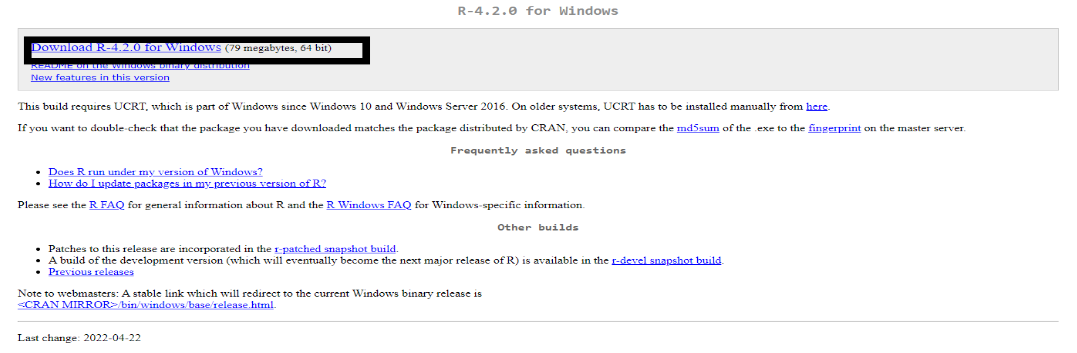
\includegraphics[width=10cm,height=8cm]{imagenes/Paso1.png}
\caption{\label{fig0}}
\end{figure}
\item \textbf{\textit{Paso 2: }}En la pestaña anterior daremos clic en el rectángulo que se muestra, donde se nos descargar un archivo .exe, que al ejecutarlo como administrador y este nos mostrara  la siguiente ventana, donde  elegiremos el idioma y aceptamos la elección:
\begin{figure}[H]
\centering
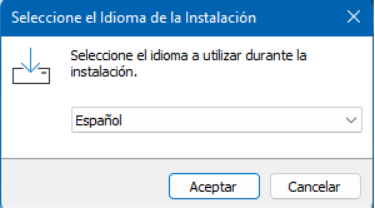
\includegraphics[width=10cm,height=7cm]{imagenes/Paso2.png}
\caption{\label{fig1}}
\end{figure}
\item \textbf{\textit{Paso 3: }}  Luego de aceptar en la ventana anterior aparecerá una nueva ventana a la cual le daremos en el botón de siguiente:
\begin{figure}[H]
\centering
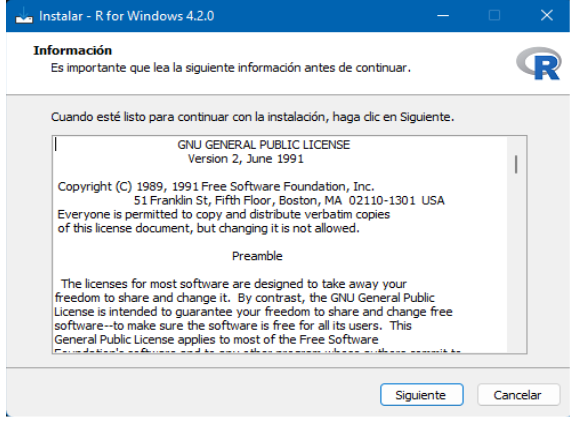
\includegraphics[width=10cm,height=5cm]{imagenes/Paso3.png}
\caption{\label{fig2}}
\end{figure}
   
\item \textbf{\textit{Paso 4: }} A continuación elegiremos la carpeta donde queremos que se guarde la instalación de dicho programa, acompañado de un clic en el botón siguiente:
\begin{figure}[H]
\centering
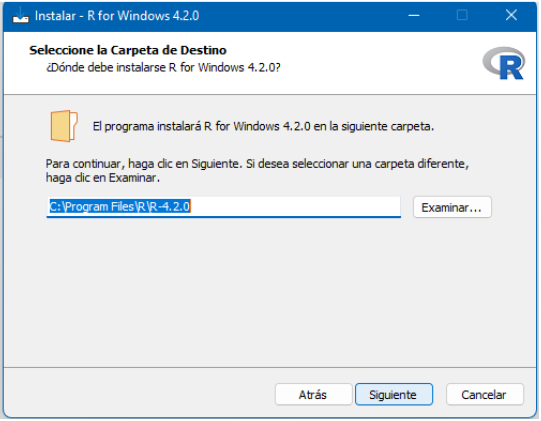
\includegraphics[width=10cm,height=5cm]{imagenes/Paso4.png}
\caption{\label{fig3}}
\end{figure}
\item \textbf{\textit{Paso 5: }}En la siguiente ventana elegiremos los componentes del programa que queremos que se descarguen, de los cuales seleccionaremos todos como se muestra en la siguiente imagen:
\begin{figure}[H]
\centering
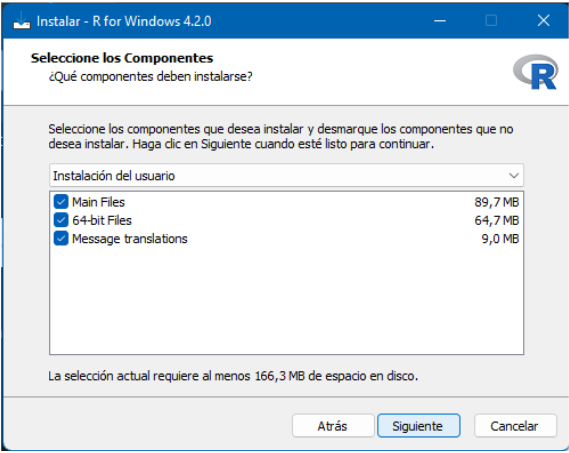
\includegraphics[width=10cm,height=5cm]{imagenes/Paso5.png}
\caption{\label{fig4}}
\end{figure}
\item \textbf{\textit{Paso 6: }}Luego especificaremos si queremos o no usar las opciones de configuración del programa:
\begin{figure}[H]
\centering
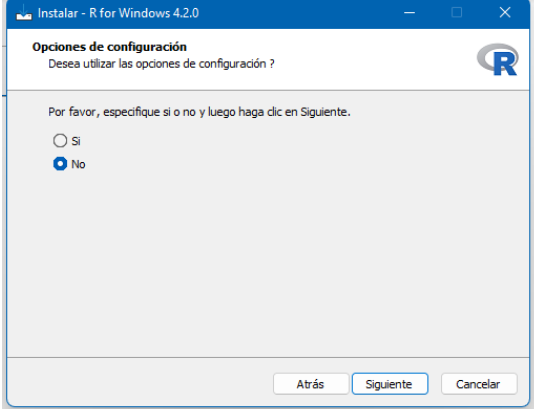
\includegraphics[width=10cm,height=5cm]{imagenes/Paso6.png}
\caption{\label{fig5}}
\end{figure}
\item \textbf{\textit{Paso 7: }}De igual forma el programa nos preguntará donde queremos que estén los accesos directos de este mismo,el cual elegiremos en el explorador de archivos :
\begin{figure}[H]
\centering
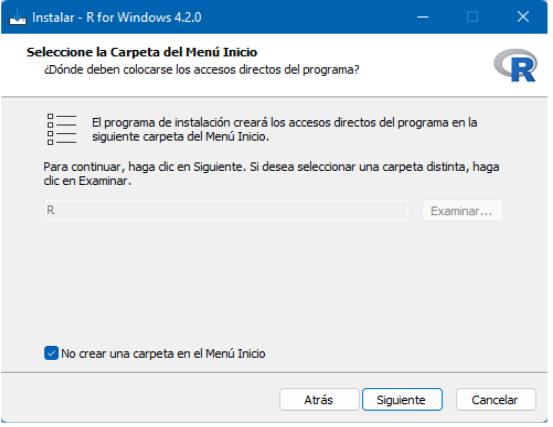
\includegraphics[width=10cm,height=5cm]{imagenes/Paso7.png}
\caption{\label{fig6}}
\end{figure}
\item \textbf{\textit{Paso 8: }}Por último el programa comenzará su instalación: 
\begin{figure}[H]
\centering
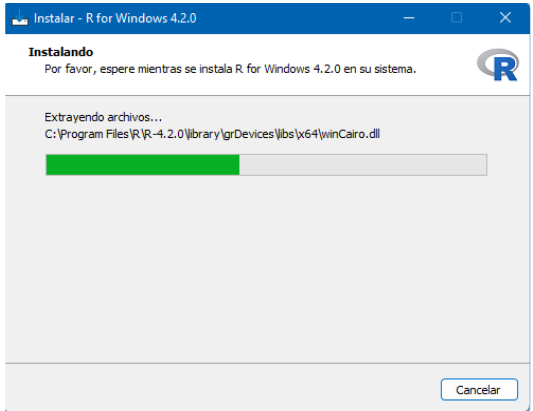
\includegraphics[width=10cm,height=5cm]{imagenes/Paso8.png}
\caption{\label{fig7}}
\end{figure}
\item \textbf{\textit{Paso 9: }}Luego de realizar todo  pasos ya tendremos R instalado localmente en nuestro computador de  confianza y listo para usar:
\begin{figure}[H]
\centering

\includegraphics[width=5cm,height=3cm]{imagenes/Paso9.png}
\caption{\label{fig8}}
\end{figure}
\end{itemize}

\section{Alternativas virtuales  de R}
Dado el caso que dispongas de un equipo que no cuente con los recursos necesarios para la instalación local de \textbf{R} o  simplemente no deseas realizar la instalación por que prefieres trabajar en la web,existen varias alternativas que te servirán para ejecutar tus códigos de manera online, algunos de estos son: \textbf{Rstudio cloud}, \textbf{Rdrr}, \textbf { jdoodle}, \textbf{ Coding Ground}.

\begin{itemize}
               %%%%%%%%%%%%%%%%%%%%%%%%%%%%%%%%%%%%%%%%%%%%%%%%%%%%%%
\item \textbf{\textit{Rstudio cloud: }}
\begin{figure}[H]
\centering

\includegraphics[width=12cm,height=7cm]{imagenes/RstudioCloud.png}
\caption{\label{fig0:frog}Vista principal de Rstudio cloud.}
\end{figure}
RStudio Cloud es una plataforma online que permite crear, ejecutar y compartir proyectos realizados en el lenguaje R, esta plataforma es de paga aunque posee también una opción gratuita(funciones un poco restringida con relación al número de proyectos que puedes realizar).\\
Para acceder a esta plataforma se debe tener una cuenta, si ya la tienes solo seria iniciar sección y empezar, de lo contrario te puedes registrar siguiendo los siguientes pasos: 
\begin{enumerate}
    \item Desde su navegador de preferencia ingrese a Rstudio cloud pinchando el siguiente link (\url{https://rstudio.cloud/}).
    \item Luego se debe hacer click el botón Sign Up que aparece en la parte superior derecha de la pantalla.
    \item Seleccione la opción \textbf{Cloud Free o cloud Premium} según prefieras
    \item Luego debes hacer clic en el botón Sign Up que aparece en la parte inferior de la pantalla
    \item Por ultimo solo seria completar el formulario  y segrí las instrucciones de registro.
\end{enumerate}
Después de esto estarías listo para usar \textbf{Rstudio Cloud}.
               %%%%%%%%%%%%%%%%%%%%%%%%%%%%%%%%%%%%%%%%%%
\item \textbf{\textit{Rdrr: }}
\begin{figure}[H]
\centering
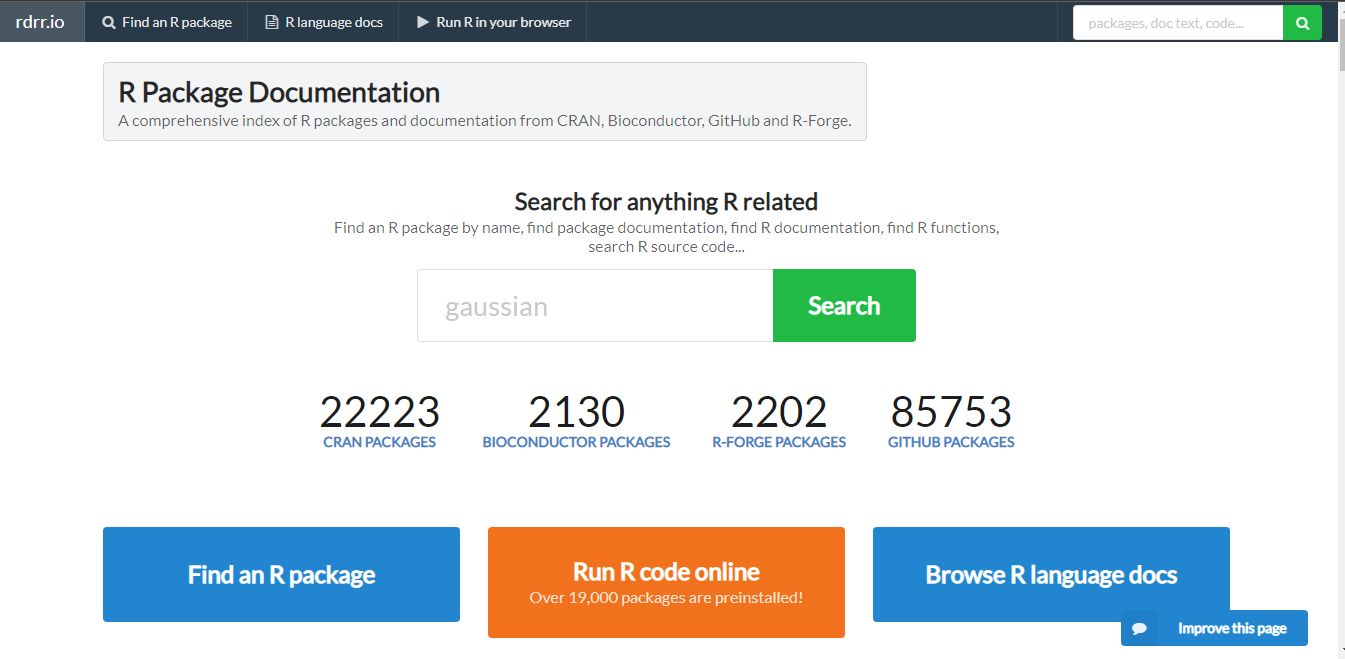
\includegraphics[width=12cm,height=7cm]{imagenes/RDRR.png}
\caption{\label{fig1:frog}Vista principal de RDRR.}
\end{figure}
Rdrr es al igual que Rstudio cloud una plataforma que permite crear y ejecutar códigos realizados el lenguaje R y además es completamente gratuita, dentro del plataforma se pueden encontrar más de diecinueve mil paquetes R precargados y bibliografía sobre el uso de los paquetes, el único inconveniente de esta plataforma es que no permite trabajar de manera colaborativa.
Para acceder no se requiere tener una cuenta y basta con seguir las siguientes instrucciones:   
\begin{enumerate}
    \item Primero pinchar el siguiente link (\url{https://rdrr.io/}), que te dirigirá a la pagina principal de la plataforma.
    \item Después eliges una de las tres opciones:
    \begin{enumerate}
        \item Find an R package.
        \item Run R code online.
        \item Browse R langueage docs.
    \end{enumerate}
\end{enumerate}
Luego de seleccionar la opción deseada y estarías listo para usar la plataforma.

                %%%%%%%%%%%%%%%%%%%%%%%%%%%%%%%%%%%%%%%%%%%%%

\item \textbf{\textit{Jdoodle: }} 
\begin{figure}[H]
\centering
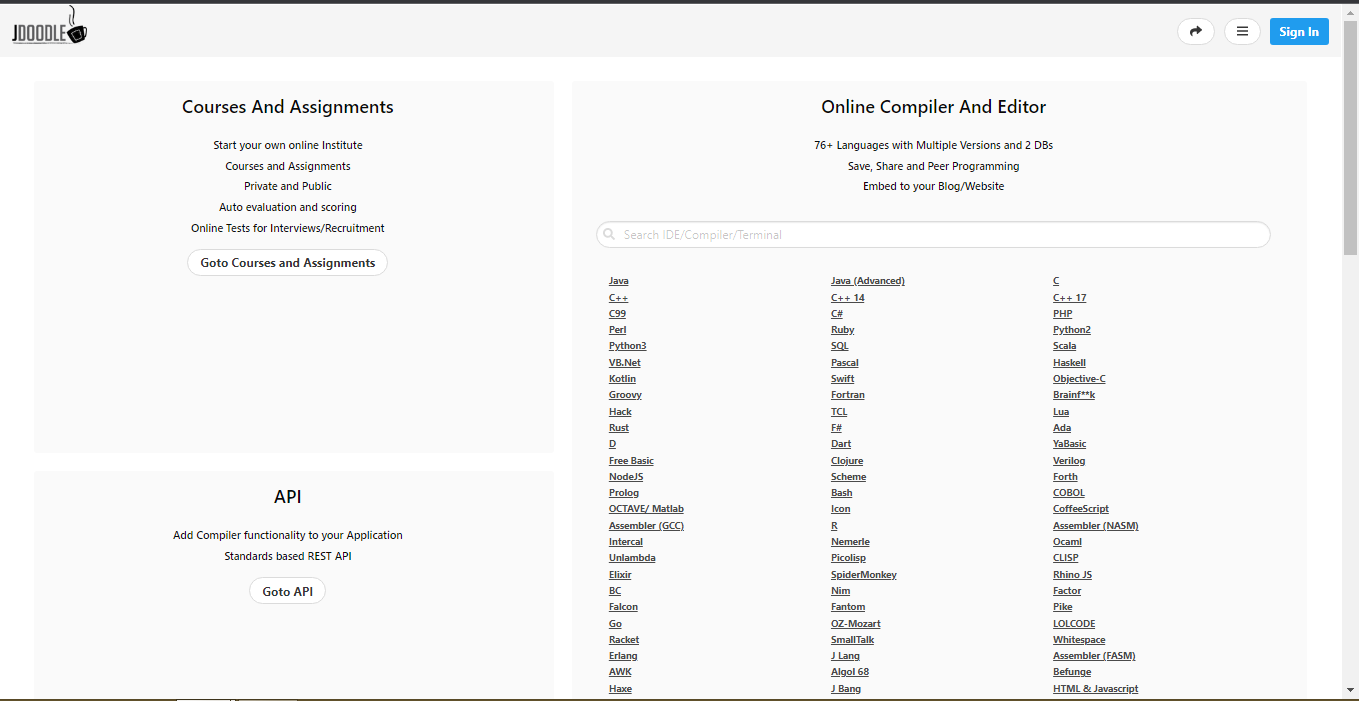
\includegraphics[width=12cm,height=7cm]{imagenes/Jdoodle.png}
\caption{\label{fig2:frog}Vista principal de Jdoodle.}
\end{figure}
Jdoodle es un compilador online con el cual puedes ejecutar código de múltiples lenguajes de programación como c, c++, java, entre otros, incluyendo el lenguaje que nos interesa  que en este caso es R. En esta plataforma puedes realizar códigos sin necesidad de registrarte o también si lo de seas puedes hacerlo.  Para hacer uso de esta plataforma hay que seguir los siguientes pasos: 
\begin{enumerate}
    \item Primero hay que acceder a la pagina principal, la cual la puedes encontrar dando clic en el siguiente link(\url{https://www.jdoodle.com/} )
    \item En segundo lugar solo seria seleccionar el lenguaje R y comenzar a programar, pero si deseas registrarte puede seguir los siguientes pasos: 
    \begin{enumerate}
        \item  Primeramente se debe hacer clic en el botón \textbf{Sign Ln} que aparece en las parte superior derecha de la pantalla.
        \item Luego seleccionar una de las opciones de registro que ofrece la plataforma las cuales son:
        \begin{enumerate}
            \item sing in with google
            \item sing in whith Microsoft
        \end{enumerate}
        \item por ultimo regresar al primer paso
    \end{enumerate}
\end{enumerate}
Seguidamente ya estarían listos para programar en R dentro de esta plataforma.

                 %%%%%%%%%%%%%%%%%%%%%%%%%%%%%%%%%%%%%%%%%%
\item \textbf{\textit{Conding Ground: }}
\begin{figure}[H]
\centering
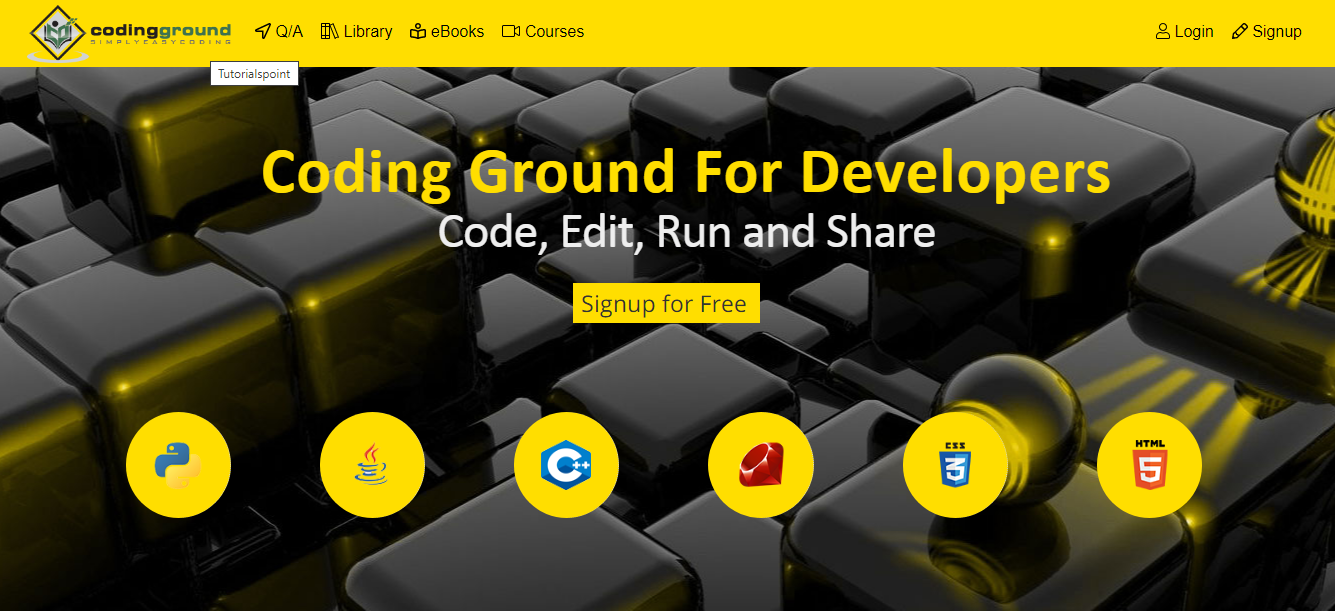
\includegraphics[width=12cm,height=7cm]{imagenes/CodingGraund.png}
\caption{\label{fig3:frog}Vista principal de Coding Ground.}
\end{figure}
Conding Ground al igual que Jdoodle es un compilador online con el cual puedes ejecutar código de múltiples lenguajes de programación incluido R. En esta plataforma también se pueden realizar códigos sin necesidad de registrarse o si lo de seas puedes hacerlo. Para hacer uso de esta plataforma puedes seguir los siguientes pasos: 
\begin{enumerate}
    \item En primer lugar hay que acceder a la pagina principal, la cual la puedes encontrar dando clic en el siguiente link(\url{https://www.tutorialspoint.com/codingground.htm} )
    \item En segundo lugar solo seria seleccionar el lenguaje R y comenzar a programar, pero si deseas registrarte puede seguir los siguientes pasos: 
    \begin{enumerate}
        \item  Primeramente se debe hacer clic en el botón \textbf{Signup for Free} que aparece en las parte superior derecha de la pantalla en el centro de la pantalla
        \item Luego rellenar el formulario que aparece.
        \item por ultimo regresar al primer paso
    \end{enumerate}
   
\end{enumerate}
\end{itemize}
\textbf{Las opciones de compilación de R online aquí expuestas  son solo unas de las tantas opciones que se pueden encontrar en la web para correr vuestros códigos de R}



\section{Estructuras de Datos Básicos de R}
\section{Estructuras de Datos Básicos de R}
Las estructuras más primitivas dentro de \textbf{R} son:  vectores, matrices y data frames.\\
A continuación se encontraran las definiciones de cada una de estas y su forma de uso.  
\begin{itemize}
\item \textbf{\textit{Vectores: }}
Un vector es la estructura de datos más sencilla en R. Un vector es una colección de uno o más datos del mismo tipo.
\begin{enumerate}
    \item Propiedades de los vectores\\
    Todos los vectores tienen tres propiedades:
    \begin{enumerate}
        \item \textbf{\textit{Tipo:}} Un vector es del mismo tipo que los datos que contiene. Si tenemos un vector que contiene datos numéricos, entonces el vector  también sera de este tipo. Los vectores son atómicos, porque solo pueden contener datos de un  tipo, no se pueden mezclar datos de diferentes tipos dentro de ellos.
       \item \textbf{\textit{Largo:}} Es el número de elementos que contiene un vector. El largo es la única dimensión que tiene esta estructura de datos.
      \item \textbf{\textit{Atributos:}}Los vectores pueden tener metadatos de muchos tipos, los cuales describen características de los datos que contienen. Todos ellos son incluidos en esta propiedad. 
    \end{enumerate}
    \item  Creación de vectores:
    \begin{itemize}
        \item En R los vectores se crean usando la función c() (combinar).
         Llamamos esta función y le damos como argumento los elementos que deseamos combinar en un vector, separados por comas.
         \begin{figure}[H]
            \centering
            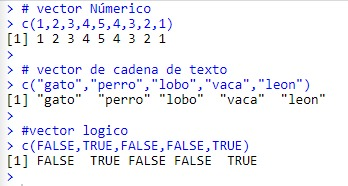
\includegraphics[width=0.5\textwidth]{imagenes/ejemplo1.jpg}
            \caption{\label{fig13}}
        \end{figure}
         \item Si deseamos agregar un elemento a un vector ya existente, podemos hacerlo combinando nuestro vector original con los elementos nuevos y asignando el resultado a nuestro vector original.
         \begin{figure}[H]
            \centering
            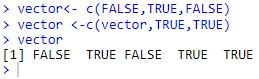
\includegraphics[width=0.5\textwidth]{imagenes/ejemplo2.jpg}
            \caption{\label{fig14}}
        \end{figure}
         \item También podemos crear vectores que son combinación de vectores.
           \begin{figure}[H]
            \centering
            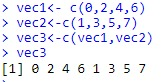
\includegraphics[width=0.5\textwidth]{imagenes/ejemplo3.jpg}
            \caption{\label{fig15}}
        \end{figure}
          \item Si intentamos combinar datos de diferentes tipos en un mismo vector, R realizará coerción automáticamente. El vector resultante será del tipo más flexible entre los datos que contenga,siguiendo las reglas de coerción.
          \begin{figure}[H]
            \centering
            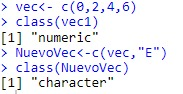
\includegraphics[width=0.5\textwidth]{imagenes/ejemplo4.jpg}
            \caption{\label{fig16}}
        \end{figure}
        
          \item se pueden crear vectores de secuencias numéricas usando :. De un lado de los dos puntos escribimos el número de inicio de la secuencia y del otro el final.\\
          Las secuencias creadas con : son consecutivas con incrementos o decrementos de 1. Estas secuencias pueden empezar con cualquier número, incluso si este es negativo o tiene cifras decimales
           \begin{figure}[H]
            \centering
            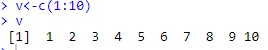
\includegraphics[width=0.5\textwidth]{imagenes/ejemplo5.jpg}
            \caption{\label{fig17}}
        \end{figure}
        
    \end{itemize}
    \item Operaciones con vectores:
    Existen algunas operaciones al aplicarlas a un vector, se aplican a cada uno de sus elementos. A este proceso le llamamos vectorización.
    Las operaciones aritméticas y relacionales pueden vectorizarse. Si las aplicamos a un vector, la operación se realizará para cada uno de los elementos que contiene
   \begin{figure}[H]
            \centering
            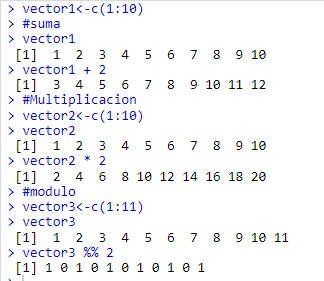
\includegraphics[width=0.5\textwidth]{imagenes/ejemplo.jpg}
            \caption{\label{fig18}}
        \end{figure}
        
\end{enumerate}

\item \textbf{\textit{Matrices: }}
Las matrices  pueden ser descritas como vectores multidimensionales. Al igual que un vector, únicamente pueden contener datos de un sólo tipo, pero además de largo, tienen más dimensiones.\\
En un sentido estricto, las matrices son una caso especial de un array, que se distingue por tener específicamente dos dimensiones, un “largo”" y un “alto”. Las matrices son, por lo tanto, una estructura con forma rectangular, con renglones y columnas.\\
Como las matrices son usadas de manera regular en matemáticas y estadística, es una estructura de datos de uso común en R común.
\begin{enumerate}
    \item  Creación de Matrices
    \begin{itemize}
        \item Creamos matrices en R con la función matrix(). La función matrix() acepta dos argumentos, nrow y ncol. Con ellos especificamos el número de renglones y columnas que tendrá nuestra matriz.
         
        \item Los datos que intentemos agrupar en una matriz serán acomodados en orden, de arriba a abajo, y de izquierda a derecha, hasta formar un rectángulo.
    \textbf{\textit{Colocar un ejemplo}}
    \item Si multiplicamos el número de renglones por el número de columnas, obtendremos el número de celdas de la matriz.
        \item Ejemplo:
        \begin{figure}[H]
            \centering
            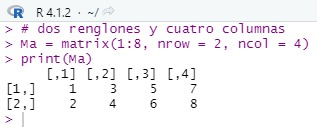
\includegraphics[width=10cm,height=5cm]{imagenes/ejemplo6.jpg}
            \caption{\label{fig19}}
        \end{figure}
      \end{itemize}
    
\end{enumerate}

\item \textbf{\textit{Data Frames: }} 
    Los data frames son estructuras de datos de dos dimensiones
    (rectangulares) que pueden contener datos de diferentes tipos, por lo tanto, son heterogéneas. Esta estructura de datos es la más usada para realizar análisis de datos
    \begin{enumerate}
            \item Se puede entender a los data frames como una versión más flexible de una matriz. Mientras que en una matriz todas las celdas deben contener datos del mismo tipo, los renglones de un data frame admiten datos de distintos tipos, pero sus columnas conservan la restricción de contener datos de un sólo tipo.
             Un data frame está compuesto por vectores. Debido a esto podemos asignar un nombre a cada vector, que se convertirá en el nombre de la columna. Como todos los nombres, es recomendable que este sea claro, no ambiguo y descriptivo
            \begin{figure}[H]
            \centering
            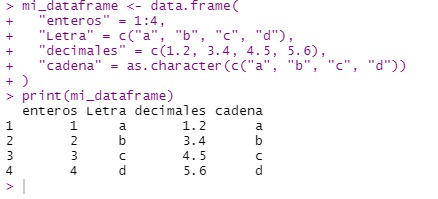
\includegraphics[width=0.5\textwidth]{imagenes/ejemplo8.jpg}
            \caption{\label{fig20}}
        \end{figure}
        
            
            \item propiedades de los Data Frames
            \begin{enumerate}
                \item Al igual que con una matriz, si aplicamos una operación aritmética a un data frame, esta se vectorizará. Los resultados que obtendremos dependerán del tipo de datos de cada columna. R nos devolverá todas las advertencias que ocurran como resultado de las operaciones realizadas, por ejemplo, aquellas que hayan requerido una coerción. 
                \begin{figure}[H]
            \centering
            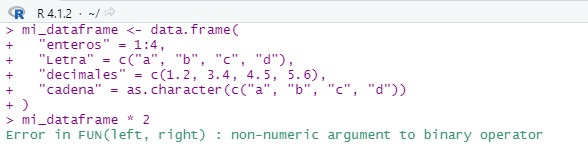
\includegraphics[width=0.5\textwidth]{imagenes/ejemplo7.jpg}
            \caption{\label{fig21}}
        \end{figure}
        
              
            \end{enumerate}
        \end{enumerate}
\end{itemize}


\section{Visualización de datos en R}
Compruebe que la ventana R interactivo funciona escribiendo $3 + 4$ y luego presionando \textbf{Entrar} para ver el resultado:
\begin{center}
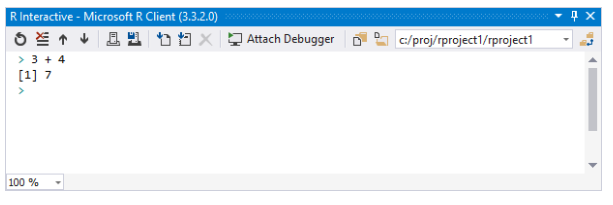
\includegraphics[width=0.5\textwidth]{anúgwe/C1.PNG}
\end{center}
 Escriba algo un poco más complicado, \textbf{ds} $< - c$ (1.5, 6.7, 8.9) * 1:12, y luego escriba \textbf{ds} para ver el resultado:
\begin{center}
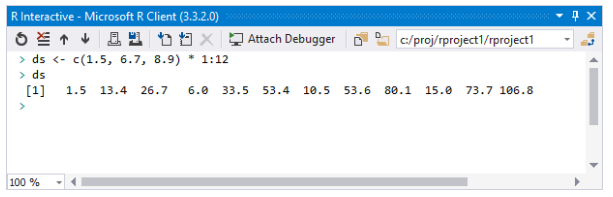
\includegraphics[width=0.5\textwidth]{anúgwe/C2.PNG}
\end{center}
 Escriba \textbf{mean(ds)} pero tenga en cuenta que tan pronto como escriba \textbf{m $o$ me}, Visual Studio IntelliSense proporciona opciones de Autocompletar. Cuando la opción de Autocompletar que quiera esté seleccionada en la lista, presione \textbf{Tab} para insertarla:
  \begin{center}
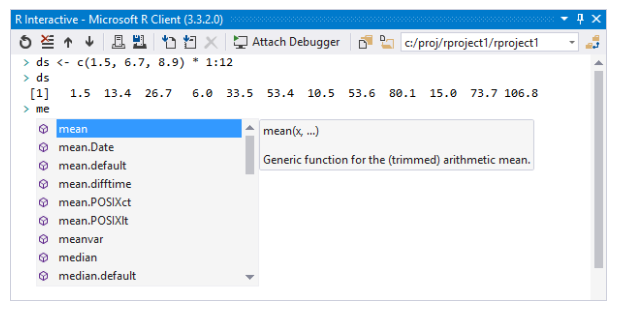
\includegraphics[width=0.5\textwidth]{anúgwe/C3.PNG}
\end{center}
Después de completar \textbf{mean}, escriba el paréntesis de apertura ( y observe cómo IntelliSense proporciona ayuda en línea para la función:
\begin{center}
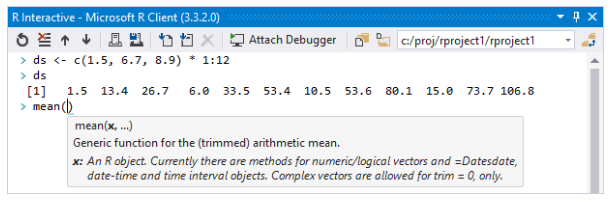
\includegraphics[width=0.5\textwidth]{anúgwe/C4.PNG}
\end{center}
Complete la línea \textbf{mean(ds)} y presione Entrar para ver el resultado ([1] 39.51667).
\\

Algunos comandos, como \textbf{plot(1:100)}, abren una nueva ventana en Visual Studio cuando los resultados no se pueden mostrar directamente en la ventana interactiva:
\begin{center}
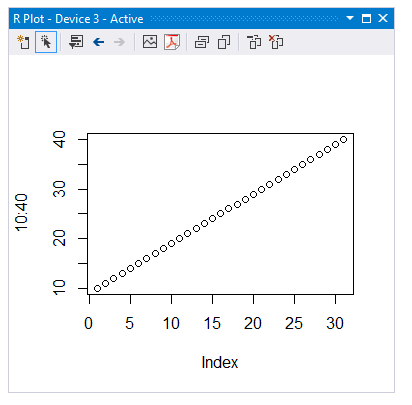
\includegraphics[width=0.5\textwidth]{anúgwe/C5.PNG}
\end{center}
La ventana interactiva también permite revisar el historial, cargar y guardar áreas de trabajo, adjuntar e interactuar con los archivos de código fuente en lugar de usar las operaciones.\\


\section{Referencias}
\begin{itemize}
    \item Vega, J. B. M. (n.d.). R para principiantes. \url{Bookdown.Org.} Retrieved June 10, 2022, from \url{https://bookdown.org/jboscomendoza/r-principiantes4/matrices-y-arrays.html}
    \item Vega, J. B. M. (n.d.). R para principiantes.
    \url{Bookdown.Org.}  Retrieved June 10, 2022, from \url{https://bookdown.org/jboscomendoza/r-principiantes4/vectores.html}
    \item Vega, J. B. M. (n.d.). R para principiantes.
    \url{Bookdown.Org.} Retrieved June 10, 2022, from \url{https://bookdown.org/jboscomendoza/r-principiantes4/data-frames.html}
    \item Tutorial de introducción a R - Visual Studio (Windows). (n.d.).
    \url{Microsoft.com.} Retrieved June 12, 2022, from \url{https://docs.microsoft.com/es-es/visualstudio/rtvs/getting-started-with-r?view=vs-2017}
    \item (N.d.).
    \url{Tutorialspoint.Com.} Retrieved June 12, 2022, from \url{https://www.tutorialspoint.com/r/r_tutorial.pdf}
    \item R-4.2.0 for Windows. (n.d.). 
    \url{R-Project.Org.} Retrieved June 12, 2022, from 
    \url{https://cran.r-project.org/bin/windows/base/}
\end{itemize}
\end{document}